% Created by tikzDevice version 0.12.3.1 on 2021-04-04 18:35:02
% !TEX encoding = UTF-8 Unicode
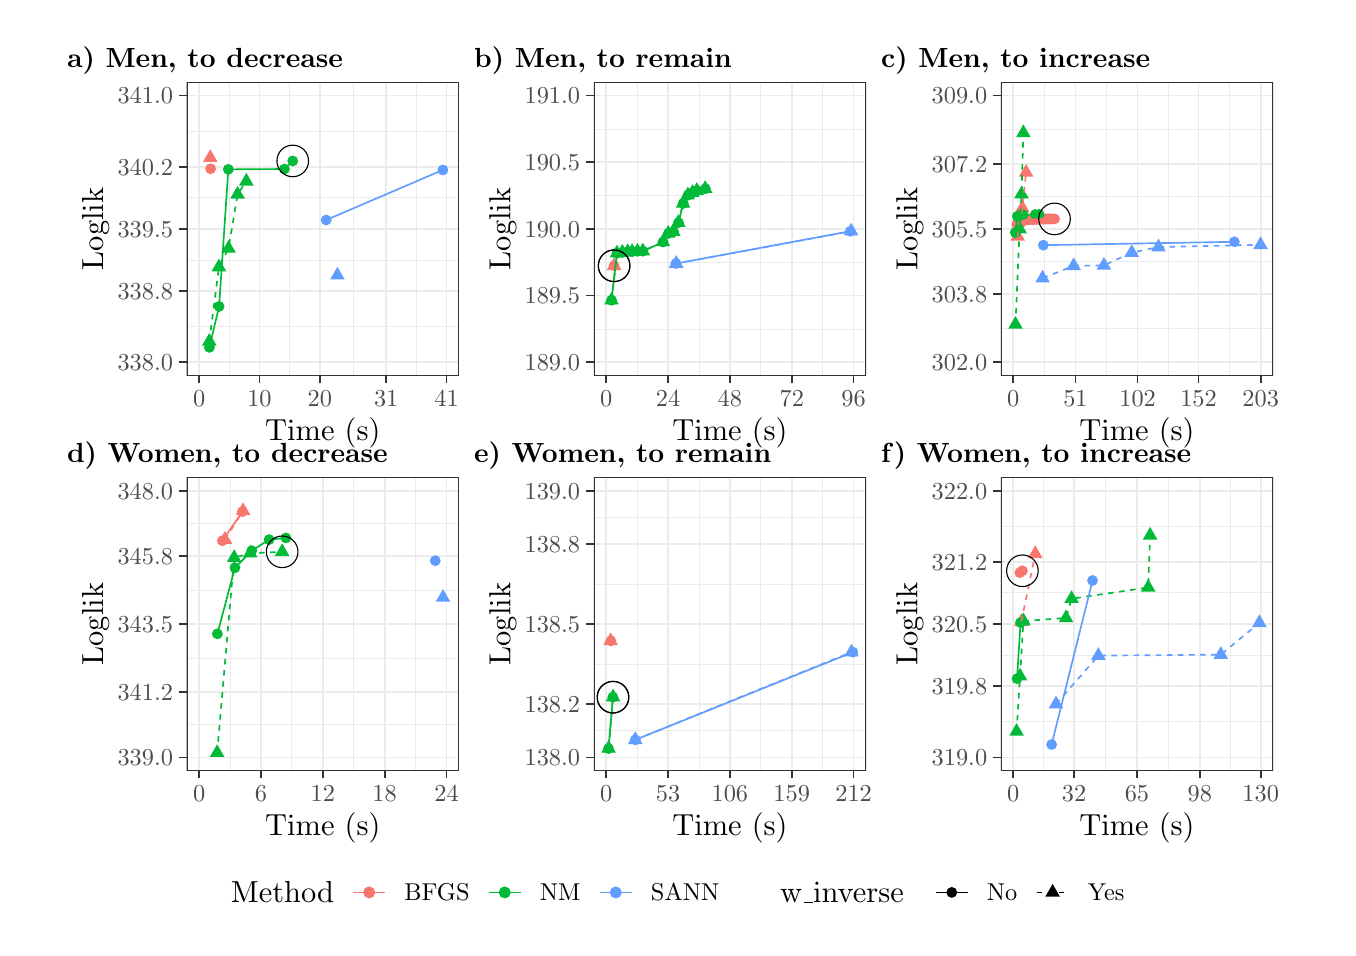
\begin{tikzpicture}[x=1pt,y=1pt]
\definecolor{fillColor}{RGB}{255,255,255}
\path[use as bounding box,fill=fillColor,fill opacity=0.00] (0,0) rectangle (469.75,325.21);
\begin{scope}
\path[clip] ( 14.23,168.22) rectangle (161.33,310.99);
\definecolor{drawColor}{RGB}{255,255,255}
\definecolor{fillColor}{RGB}{255,255,255}

\path[draw=drawColor,line width= 0.6pt,line join=round,line cap=round,fill=fillColor] ( 14.23,168.22) rectangle (161.33,310.99);
\end{scope}
\begin{scope}
\path[clip] ( 57.47,199.47) rectangle (155.83,305.49);
\definecolor{fillColor}{RGB}{255,255,255}

\path[fill=fillColor] ( 57.47,199.47) rectangle (155.83,305.49);
\definecolor{drawColor}{gray}{0.92}

\path[draw=drawColor,line width= 0.3pt,line join=round] ( 57.47,217.14) --
	(155.83,217.14);

\path[draw=drawColor,line width= 0.3pt,line join=round] ( 57.47,241.24) --
	(155.83,241.24);

\path[draw=drawColor,line width= 0.3pt,line join=round] ( 57.47,263.73) --
	(155.83,263.73);

\path[draw=drawColor,line width= 0.3pt,line join=round] ( 57.47,287.82) --
	(155.83,287.82);

\path[draw=drawColor,line width= 0.3pt,line join=round] ( 72.85,199.47) --
	( 72.85,305.49);

\path[draw=drawColor,line width= 0.3pt,line join=round] ( 94.65,199.47) --
	( 94.65,305.49);

\path[draw=drawColor,line width= 0.3pt,line join=round] (117.55,199.47) --
	(117.55,305.49);

\path[draw=drawColor,line width= 0.3pt,line join=round] (140.45,199.47) --
	(140.45,305.49);

\path[draw=drawColor,line width= 0.6pt,line join=round] ( 57.47,204.29) --
	(155.83,204.29);

\path[draw=drawColor,line width= 0.6pt,line join=round] ( 57.47,229.99) --
	(155.83,229.99);

\path[draw=drawColor,line width= 0.6pt,line join=round] ( 57.47,252.48) --
	(155.83,252.48);

\path[draw=drawColor,line width= 0.6pt,line join=round] ( 57.47,274.97) --
	(155.83,274.97);

\path[draw=drawColor,line width= 0.6pt,line join=round] ( 57.47,300.67) --
	(155.83,300.67);

\path[draw=drawColor,line width= 0.6pt,line join=round] ( 61.94,199.47) --
	( 61.94,305.49);

\path[draw=drawColor,line width= 0.6pt,line join=round] ( 83.75,199.47) --
	( 83.75,305.49);

\path[draw=drawColor,line width= 0.6pt,line join=round] (105.56,199.47) --
	(105.56,305.49);

\path[draw=drawColor,line width= 0.6pt,line join=round] (129.55,199.47) --
	(129.55,305.49);

\path[draw=drawColor,line width= 0.6pt,line join=round] (151.36,199.47) --
	(151.36,305.49);
\definecolor{fillColor}{RGB}{248,118,109}

\path[fill=fillColor] ( 66.09,274.23) circle (  1.96);

\path[fill=fillColor] ( 65.98,281.26) --
	( 68.63,276.69) --
	( 63.34,276.69) --
	cycle;
\definecolor{fillColor}{RGB}{0,186,56}

\path[fill=fillColor] ( 65.67,209.68) circle (  1.96);

\path[fill=fillColor] ( 69.17,224.48) circle (  1.96);

\path[fill=fillColor] ( 72.51,274.00) circle (  1.96);

\path[fill=fillColor] ( 92.78,274.13) circle (  1.96);

\path[fill=fillColor] ( 95.78,277.05) circle (  1.96);

\path[fill=fillColor] ( 65.63,214.90) --
	( 68.28,210.32) --
	( 62.99,210.32) --
	cycle;

\path[fill=fillColor] ( 69.11,241.77) --
	( 71.76,237.19) --
	( 66.47,237.19) --
	cycle;

\path[fill=fillColor] ( 72.58,248.49) --
	( 75.23,243.91) --
	( 69.94,243.91) --
	cycle;

\path[fill=fillColor] ( 75.84,268.02) --
	( 78.48,263.44) --
	( 73.20,263.44) --
	cycle;

\path[fill=fillColor] ( 79.02,272.75) --
	( 81.66,268.17) --
	( 76.38,268.17) --
	cycle;
\definecolor{fillColor}{RGB}{97,156,255}

\path[fill=fillColor] (107.87,255.71) circle (  1.96);

\path[fill=fillColor] (150.04,273.80) circle (  1.96);

\path[fill=fillColor] (111.93,238.78) --
	(114.57,234.21) --
	(109.29,234.21) --
	cycle;
\definecolor{drawColor}{RGB}{0,186,56}

\path[draw=drawColor,line width= 0.6pt,line join=round] ( 65.67,209.68) --
	( 69.17,224.48) --
	( 72.51,274.00) --
	( 92.78,274.13) --
	( 95.78,277.05);

\path[draw=drawColor,line width= 0.6pt,dash pattern=on 2pt off 2pt ,line join=round] ( 65.63,211.85) --
	( 69.11,238.72) --
	( 72.58,245.44) --
	( 75.84,264.96) --
	( 79.02,269.70);
\definecolor{drawColor}{RGB}{97,156,255}

\path[draw=drawColor,line width= 0.6pt,line join=round] (107.87,255.71) --
	(150.04,273.80);
\definecolor{drawColor}{RGB}{0,0,0}

\path[draw=drawColor,line width= 0.4pt,line join=round,line cap=round] ( 95.78,277.05) circle (  5.71);
\definecolor{drawColor}{gray}{0.20}

\path[draw=drawColor,line width= 0.6pt,line join=round,line cap=round] ( 57.47,199.47) rectangle (155.83,305.49);
\end{scope}
\begin{scope}
\path[clip] (  0.00,  0.00) rectangle (469.75,325.21);
\definecolor{drawColor}{gray}{0.30}

\node[text=drawColor,anchor=base east,inner sep=0pt, outer sep=0pt, scale=  0.88] at ( 52.52,201.26) {338.0};

\node[text=drawColor,anchor=base east,inner sep=0pt, outer sep=0pt, scale=  0.88] at ( 52.52,226.96) {338.8};

\node[text=drawColor,anchor=base east,inner sep=0pt, outer sep=0pt, scale=  0.88] at ( 52.52,249.45) {339.5};

\node[text=drawColor,anchor=base east,inner sep=0pt, outer sep=0pt, scale=  0.88] at ( 52.52,271.94) {340.2};

\node[text=drawColor,anchor=base east,inner sep=0pt, outer sep=0pt, scale=  0.88] at ( 52.52,297.64) {341.0};
\end{scope}
\begin{scope}
\path[clip] (  0.00,  0.00) rectangle (469.75,325.21);
\definecolor{drawColor}{gray}{0.20}

\path[draw=drawColor,line width= 0.6pt,line join=round] ( 54.72,204.29) --
	( 57.47,204.29);

\path[draw=drawColor,line width= 0.6pt,line join=round] ( 54.72,229.99) --
	( 57.47,229.99);

\path[draw=drawColor,line width= 0.6pt,line join=round] ( 54.72,252.48) --
	( 57.47,252.48);

\path[draw=drawColor,line width= 0.6pt,line join=round] ( 54.72,274.97) --
	( 57.47,274.97);

\path[draw=drawColor,line width= 0.6pt,line join=round] ( 54.72,300.67) --
	( 57.47,300.67);
\end{scope}
\begin{scope}
\path[clip] (  0.00,  0.00) rectangle (469.75,325.21);
\definecolor{drawColor}{gray}{0.20}

\path[draw=drawColor,line width= 0.6pt,line join=round] ( 61.94,196.72) --
	( 61.94,199.47);

\path[draw=drawColor,line width= 0.6pt,line join=round] ( 83.75,196.72) --
	( 83.75,199.47);

\path[draw=drawColor,line width= 0.6pt,line join=round] (105.56,196.72) --
	(105.56,199.47);

\path[draw=drawColor,line width= 0.6pt,line join=round] (129.55,196.72) --
	(129.55,199.47);

\path[draw=drawColor,line width= 0.6pt,line join=round] (151.36,196.72) --
	(151.36,199.47);
\end{scope}
\begin{scope}
\path[clip] (  0.00,  0.00) rectangle (469.75,325.21);
\definecolor{drawColor}{gray}{0.30}

\node[text=drawColor,anchor=base,inner sep=0pt, outer sep=0pt, scale=  0.88] at ( 61.94,188.46) {0};

\node[text=drawColor,anchor=base,inner sep=0pt, outer sep=0pt, scale=  0.88] at ( 83.75,188.46) {10};

\node[text=drawColor,anchor=base,inner sep=0pt, outer sep=0pt, scale=  0.88] at (105.56,188.46) {20};

\node[text=drawColor,anchor=base,inner sep=0pt, outer sep=0pt, scale=  0.88] at (129.55,188.46) {31};

\node[text=drawColor,anchor=base,inner sep=0pt, outer sep=0pt, scale=  0.88] at (151.36,188.46) {41};
\end{scope}
\begin{scope}
\path[clip] (  0.00,  0.00) rectangle (469.75,325.21);
\definecolor{drawColor}{RGB}{0,0,0}

\node[text=drawColor,anchor=base,inner sep=0pt, outer sep=0pt, scale=  1.10] at (106.65,176.15) {Time (s)};
\end{scope}
\begin{scope}
\path[clip] (  0.00,  0.00) rectangle (469.75,325.21);
\definecolor{drawColor}{RGB}{0,0,0}

\node[text=drawColor,rotate= 90.00,anchor=base,inner sep=0pt, outer sep=0pt, scale=  1.10] at ( 27.30,252.48) {Loglik};
\end{scope}
\begin{scope}
\path[clip] (  0.00,  0.00) rectangle (469.75,325.21);
\definecolor{drawColor}{RGB}{0,0,0}

\node[text=drawColor,anchor=base west,inner sep=0pt, outer sep=0pt, scale=  1.00] at ( 14.23,310.99) {\bfseries a) Men, to decrease};
\end{scope}
\begin{scope}
\path[clip] (161.33,168.22) rectangle (308.43,310.99);
\definecolor{drawColor}{RGB}{255,255,255}
\definecolor{fillColor}{RGB}{255,255,255}

\path[draw=drawColor,line width= 0.6pt,line join=round,line cap=round,fill=fillColor] (161.33,168.22) rectangle (308.43,310.99);
\end{scope}
\begin{scope}
\path[clip] (204.57,199.47) rectangle (302.93,305.49);
\definecolor{fillColor}{RGB}{255,255,255}

\path[fill=fillColor] (204.57,199.47) rectangle (302.93,305.49);
\definecolor{drawColor}{gray}{0.92}

\path[draw=drawColor,line width= 0.3pt,line join=round] (204.57,216.34) --
	(302.93,216.34);

\path[draw=drawColor,line width= 0.3pt,line join=round] (204.57,240.43) --
	(302.93,240.43);

\path[draw=drawColor,line width= 0.3pt,line join=round] (204.57,264.53) --
	(302.93,264.53);

\path[draw=drawColor,line width= 0.3pt,line join=round] (204.57,288.62) --
	(302.93,288.62);

\path[draw=drawColor,line width= 0.3pt,line join=round] (220.22,199.47) --
	(220.22,305.49);

\path[draw=drawColor,line width= 0.3pt,line join=round] (242.57,199.47) --
	(242.57,305.49);

\path[draw=drawColor,line width= 0.3pt,line join=round] (264.93,199.47) --
	(264.93,305.49);

\path[draw=drawColor,line width= 0.3pt,line join=round] (287.28,199.47) --
	(287.28,305.49);

\path[draw=drawColor,line width= 0.6pt,line join=round] (204.57,204.29) --
	(302.93,204.29);

\path[draw=drawColor,line width= 0.6pt,line join=round] (204.57,228.39) --
	(302.93,228.39);

\path[draw=drawColor,line width= 0.6pt,line join=round] (204.57,252.48) --
	(302.93,252.48);

\path[draw=drawColor,line width= 0.6pt,line join=round] (204.57,276.58) --
	(302.93,276.58);

\path[draw=drawColor,line width= 0.6pt,line join=round] (204.57,300.67) --
	(302.93,300.67);

\path[draw=drawColor,line width= 0.6pt,line join=round] (209.04,199.47) --
	(209.04,305.49);

\path[draw=drawColor,line width= 0.6pt,line join=round] (231.40,199.47) --
	(231.40,305.49);

\path[draw=drawColor,line width= 0.6pt,line join=round] (253.75,199.47) --
	(253.75,305.49);

\path[draw=drawColor,line width= 0.6pt,line join=round] (276.10,199.47) --
	(276.10,305.49);

\path[draw=drawColor,line width= 0.6pt,line join=round] (298.46,199.47) --
	(298.46,305.49);
\definecolor{fillColor}{RGB}{248,118,109}

\path[fill=fillColor] (211.92,239.17) circle (  1.96);

\path[fill=fillColor] (211.90,242.22) --
	(214.55,237.64) --
	(209.26,237.64) --
	cycle;
\definecolor{fillColor}{RGB}{0,186,56}

\path[fill=fillColor] (210.98,226.71) circle (  1.96);

\path[fill=fillColor] (212.96,243.72) circle (  1.96);

\path[fill=fillColor] (214.90,244.01) circle (  1.96);

\path[fill=fillColor] (216.84,244.24) circle (  1.96);

\path[fill=fillColor] (218.42,244.27) circle (  1.96);

\path[fill=fillColor] (220.38,244.41) circle (  1.96);

\path[fill=fillColor] (222.33,244.45) circle (  1.96);

\path[fill=fillColor] (229.59,247.76) circle (  1.96);

\path[fill=fillColor] (231.51,250.84) circle (  1.96);

\path[fill=fillColor] (233.38,251.47) circle (  1.96);

\path[fill=fillColor] (235.16,254.76) circle (  1.96);

\path[fill=fillColor] (236.88,261.70) circle (  1.96);

\path[fill=fillColor] (238.60,264.67) circle (  1.96);

\path[fill=fillColor] (240.28,265.59) circle (  1.96);

\path[fill=fillColor] (241.86,266.32) circle (  1.96);

\path[fill=fillColor] (244.90,267.01) circle (  1.96);

\path[fill=fillColor] (210.97,229.77) --
	(213.62,225.19) --
	(208.33,225.19) --
	cycle;

\path[fill=fillColor] (212.95,246.78) --
	(215.60,242.20) --
	(210.31,242.20) --
	cycle;

\path[fill=fillColor] (214.89,247.06) --
	(217.53,242.48) --
	(212.25,242.48) --
	cycle;

\path[fill=fillColor] (216.82,247.29) --
	(219.47,242.71) --
	(214.18,242.71) --
	cycle;

\path[fill=fillColor] (218.41,247.32) --
	(221.05,242.74) --
	(215.76,242.74) --
	cycle;

\path[fill=fillColor] (220.36,247.46) --
	(223.00,242.89) --
	(217.72,242.89) --
	cycle;

\path[fill=fillColor] (222.30,247.50) --
	(224.94,242.92) --
	(219.66,242.92) --
	cycle;

\path[fill=fillColor] (229.55,250.81) --
	(232.19,246.24) --
	(226.91,246.24) --
	cycle;

\path[fill=fillColor] (231.47,253.89) --
	(234.11,249.32) --
	(228.83,249.32) --
	cycle;

\path[fill=fillColor] (233.33,254.52) --
	(235.97,249.95) --
	(230.69,249.95) --
	cycle;

\path[fill=fillColor] (235.11,257.81) --
	(237.76,253.23) --
	(232.47,253.23) --
	cycle;

\path[fill=fillColor] (236.83,264.76) --
	(239.47,260.18) --
	(234.19,260.18) --
	cycle;

\path[fill=fillColor] (238.54,267.73) --
	(241.18,263.15) --
	(235.90,263.15) --
	cycle;

\path[fill=fillColor] (240.21,268.64) --
	(242.85,264.07) --
	(237.57,264.07) --
	cycle;

\path[fill=fillColor] (241.79,269.37) --
	(244.44,264.79) --
	(239.15,264.79) --
	cycle;

\path[fill=fillColor] (244.83,270.06) --
	(247.47,265.48) --
	(242.19,265.48) --
	cycle;
\definecolor{fillColor}{RGB}{97,156,255}

\path[fill=fillColor] (234.24,239.97) circle (  1.96);

\path[fill=fillColor] (297.27,251.65) circle (  1.96);

\path[fill=fillColor] (234.33,243.02) --
	(236.98,238.45) --
	(231.69,238.45) --
	cycle;

\path[fill=fillColor] (297.57,254.70) --
	(300.21,250.12) --
	(294.93,250.12) --
	cycle;
\definecolor{drawColor}{RGB}{0,186,56}

\path[draw=drawColor,line width= 0.6pt,line join=round] (210.98,226.71) --
	(212.96,243.72) --
	(214.90,244.01) --
	(216.84,244.24) --
	(218.42,244.27) --
	(220.38,244.41) --
	(222.33,244.45) --
	(229.59,247.76) --
	(231.51,250.84) --
	(233.38,251.47) --
	(235.16,254.76) --
	(236.88,261.70) --
	(238.60,264.67) --
	(240.28,265.59) --
	(241.86,266.32) --
	(244.90,267.01);

\path[draw=drawColor,line width= 0.6pt,dash pattern=on 2pt off 2pt ,line join=round] (210.97,226.71) --
	(212.95,243.72) --
	(214.89,244.01) --
	(216.82,244.24) --
	(218.41,244.27) --
	(220.36,244.41) --
	(222.30,244.45) --
	(229.55,247.76) --
	(231.47,250.84) --
	(233.33,251.47) --
	(235.11,254.76) --
	(236.83,261.70) --
	(238.54,264.67) --
	(240.21,265.59) --
	(241.79,266.32) --
	(244.83,267.01);
\definecolor{drawColor}{RGB}{97,156,255}

\path[draw=drawColor,line width= 0.6pt,line join=round] (234.24,239.97) --
	(297.27,251.65);

\path[draw=drawColor,line width= 0.6pt,dash pattern=on 2pt off 2pt ,line join=round] (234.33,239.97) --
	(297.57,251.65);
\definecolor{drawColor}{RGB}{0,0,0}

\path[draw=drawColor,line width= 0.4pt,line join=round,line cap=round] (211.92,239.17) circle (  5.71);

\path[draw=drawColor,line width= 0.4pt,line join=round,line cap=round] (211.90,239.17) circle (  5.71);
\definecolor{drawColor}{gray}{0.20}

\path[draw=drawColor,line width= 0.6pt,line join=round,line cap=round] (204.57,199.47) rectangle (302.93,305.49);
\end{scope}
\begin{scope}
\path[clip] (  0.00,  0.00) rectangle (469.75,325.21);
\definecolor{drawColor}{gray}{0.30}

\node[text=drawColor,anchor=base east,inner sep=0pt, outer sep=0pt, scale=  0.88] at (199.62,201.26) {189.0};

\node[text=drawColor,anchor=base east,inner sep=0pt, outer sep=0pt, scale=  0.88] at (199.62,225.36) {189.5};

\node[text=drawColor,anchor=base east,inner sep=0pt, outer sep=0pt, scale=  0.88] at (199.62,249.45) {190.0};

\node[text=drawColor,anchor=base east,inner sep=0pt, outer sep=0pt, scale=  0.88] at (199.62,273.55) {190.5};

\node[text=drawColor,anchor=base east,inner sep=0pt, outer sep=0pt, scale=  0.88] at (199.62,297.64) {191.0};
\end{scope}
\begin{scope}
\path[clip] (  0.00,  0.00) rectangle (469.75,325.21);
\definecolor{drawColor}{gray}{0.20}

\path[draw=drawColor,line width= 0.6pt,line join=round] (201.82,204.29) --
	(204.57,204.29);

\path[draw=drawColor,line width= 0.6pt,line join=round] (201.82,228.39) --
	(204.57,228.39);

\path[draw=drawColor,line width= 0.6pt,line join=round] (201.82,252.48) --
	(204.57,252.48);

\path[draw=drawColor,line width= 0.6pt,line join=round] (201.82,276.58) --
	(204.57,276.58);

\path[draw=drawColor,line width= 0.6pt,line join=round] (201.82,300.67) --
	(204.57,300.67);
\end{scope}
\begin{scope}
\path[clip] (  0.00,  0.00) rectangle (469.75,325.21);
\definecolor{drawColor}{gray}{0.20}

\path[draw=drawColor,line width= 0.6pt,line join=round] (209.04,196.72) --
	(209.04,199.47);

\path[draw=drawColor,line width= 0.6pt,line join=round] (231.40,196.72) --
	(231.40,199.47);

\path[draw=drawColor,line width= 0.6pt,line join=round] (253.75,196.72) --
	(253.75,199.47);

\path[draw=drawColor,line width= 0.6pt,line join=round] (276.10,196.72) --
	(276.10,199.47);

\path[draw=drawColor,line width= 0.6pt,line join=round] (298.46,196.72) --
	(298.46,199.47);
\end{scope}
\begin{scope}
\path[clip] (  0.00,  0.00) rectangle (469.75,325.21);
\definecolor{drawColor}{gray}{0.30}

\node[text=drawColor,anchor=base,inner sep=0pt, outer sep=0pt, scale=  0.88] at (209.04,188.46) {0};

\node[text=drawColor,anchor=base,inner sep=0pt, outer sep=0pt, scale=  0.88] at (231.40,188.46) {24};

\node[text=drawColor,anchor=base,inner sep=0pt, outer sep=0pt, scale=  0.88] at (253.75,188.46) {48};

\node[text=drawColor,anchor=base,inner sep=0pt, outer sep=0pt, scale=  0.88] at (276.10,188.46) {72};

\node[text=drawColor,anchor=base,inner sep=0pt, outer sep=0pt, scale=  0.88] at (298.46,188.46) {96};
\end{scope}
\begin{scope}
\path[clip] (  0.00,  0.00) rectangle (469.75,325.21);
\definecolor{drawColor}{RGB}{0,0,0}

\node[text=drawColor,anchor=base,inner sep=0pt, outer sep=0pt, scale=  1.10] at (253.75,176.15) {Time (s)};
\end{scope}
\begin{scope}
\path[clip] (  0.00,  0.00) rectangle (469.75,325.21);
\definecolor{drawColor}{RGB}{0,0,0}

\node[text=drawColor,rotate= 90.00,anchor=base,inner sep=0pt, outer sep=0pt, scale=  1.10] at (174.40,252.48) {Loglik};
\end{scope}
\begin{scope}
\path[clip] (  0.00,  0.00) rectangle (469.75,325.21);
\definecolor{drawColor}{RGB}{0,0,0}

\node[text=drawColor,anchor=base west,inner sep=0pt, outer sep=0pt, scale=  1.00] at (161.33,310.99) {\bfseries b) Men, to remain};
\end{scope}
\begin{scope}
\path[clip] (308.43,168.22) rectangle (455.53,310.99);
\definecolor{drawColor}{RGB}{255,255,255}
\definecolor{fillColor}{RGB}{255,255,255}

\path[draw=drawColor,line width= 0.6pt,line join=round,line cap=round,fill=fillColor] (308.43,168.22) rectangle (455.53,310.99);
\end{scope}
\begin{scope}
\path[clip] (351.67,199.47) rectangle (450.03,305.49);
\definecolor{fillColor}{RGB}{255,255,255}

\path[fill=fillColor] (351.67,199.47) rectangle (450.03,305.49);
\definecolor{drawColor}{gray}{0.92}

\path[draw=drawColor,line width= 0.3pt,line join=round] (351.67,216.68) --
	(450.03,216.68);

\path[draw=drawColor,line width= 0.3pt,line join=round] (351.67,240.78) --
	(450.03,240.78);

\path[draw=drawColor,line width= 0.3pt,line join=round] (351.67,264.18) --
	(450.03,264.18);

\path[draw=drawColor,line width= 0.3pt,line join=round] (351.67,288.28) --
	(450.03,288.28);

\path[draw=drawColor,line width= 0.3pt,line join=round] (367.38,199.47) --
	(367.38,305.49);

\path[draw=drawColor,line width= 0.3pt,line join=round] (389.84,199.47) --
	(389.84,305.49);

\path[draw=drawColor,line width= 0.3pt,line join=round] (412.08,199.47) --
	(412.08,305.49);

\path[draw=drawColor,line width= 0.3pt,line join=round] (434.33,199.47) --
	(434.33,305.49);

\path[draw=drawColor,line width= 0.6pt,line join=round] (351.67,204.29) --
	(450.03,204.29);

\path[draw=drawColor,line width= 0.6pt,line join=round] (351.67,229.08) --
	(450.03,229.08);

\path[draw=drawColor,line width= 0.6pt,line join=round] (351.67,252.48) --
	(450.03,252.48);

\path[draw=drawColor,line width= 0.6pt,line join=round] (351.67,275.89) --
	(450.03,275.89);

\path[draw=drawColor,line width= 0.6pt,line join=round] (351.67,300.67) --
	(450.03,300.67);

\path[draw=drawColor,line width= 0.6pt,line join=round] (356.14,199.47) --
	(356.14,305.49);

\path[draw=drawColor,line width= 0.6pt,line join=round] (378.61,199.47) --
	(378.61,305.49);

\path[draw=drawColor,line width= 0.6pt,line join=round] (401.07,199.47) --
	(401.07,305.49);

\path[draw=drawColor,line width= 0.6pt,line join=round] (423.09,199.47) --
	(423.09,305.49);

\path[draw=drawColor,line width= 0.6pt,line join=round] (445.56,199.47) --
	(445.56,305.49);
\definecolor{fillColor}{RGB}{248,118,109}

\path[fill=fillColor] (357.40,254.16) circle (  1.96);

\path[fill=fillColor] (358.11,254.61) circle (  1.96);

\path[fill=fillColor] (358.94,254.79) circle (  1.96);

\path[fill=fillColor] (359.76,255.51) circle (  1.96);

\path[fill=fillColor] (360.39,255.67) circle (  1.96);

\path[fill=fillColor] (360.99,255.78) circle (  1.96);

\path[fill=fillColor] (361.56,255.82) circle (  1.96);

\path[fill=fillColor] (362.02,255.86) circle (  1.96);

\path[fill=fillColor] (362.49,255.89) circle (  1.96);

\path[fill=fillColor] (363.01,255.92) circle (  1.96);

\path[fill=fillColor] (363.52,255.94) circle (  1.96);

\path[fill=fillColor] (364.03,255.96) circle (  1.96);

\path[fill=fillColor] (364.52,255.98) circle (  1.96);

\path[fill=fillColor] (364.99,256.00) circle (  1.96);

\path[fill=fillColor] (365.49,256.02) circle (  1.96);

\path[fill=fillColor] (366.02,256.04) circle (  1.96);

\path[fill=fillColor] (366.51,256.05) circle (  1.96);

\path[fill=fillColor] (367.00,256.06) circle (  1.96);

\path[fill=fillColor] (367.51,256.07) circle (  1.96);

\path[fill=fillColor] (368.00,256.08) circle (  1.96);

\path[fill=fillColor] (368.49,256.09) circle (  1.96);

\path[fill=fillColor] (368.99,256.09) circle (  1.96);

\path[fill=fillColor] (369.48,256.10) circle (  1.96);

\path[fill=fillColor] (369.98,256.10) circle (  1.96);

\path[fill=fillColor] (371.05,256.10) circle (  1.96);

\path[fill=fillColor] (357.73,252.84) --
	(360.37,248.27) --
	(355.09,248.27) --
	cycle;

\path[fill=fillColor] (359.41,263.07) --
	(362.06,258.50) --
	(356.77,258.50) --
	cycle;

\path[fill=fillColor] (360.78,275.95) --
	(363.43,271.38) --
	(358.14,271.38) --
	cycle;
\definecolor{fillColor}{RGB}{0,186,56}

\path[fill=fillColor] (356.87,251.17) circle (  1.96);

\path[fill=fillColor] (357.62,257.03) circle (  1.96);

\path[fill=fillColor] (358.97,257.61) circle (  1.96);

\path[fill=fillColor] (359.69,257.62) circle (  1.96);

\path[fill=fillColor] (364.12,257.71) circle (  1.96);

\path[fill=fillColor] (365.46,257.72) circle (  1.96);

\path[fill=fillColor] (356.95,221.01) --
	(359.59,216.43) --
	(354.30,216.43) --
	cycle;

\path[fill=fillColor] (358.43,255.50) --
	(361.07,250.92) --
	(355.79,250.92) --
	cycle;

\path[fill=fillColor] (359.11,268.07) --
	(361.75,263.50) --
	(356.47,263.50) --
	cycle;

\path[fill=fillColor] (359.79,290.25) --
	(362.44,285.67) --
	(357.15,285.67) --
	cycle;
\definecolor{fillColor}{RGB}{97,156,255}

\path[fill=fillColor] (367.02,246.61) circle (  1.96);

\path[fill=fillColor] (436.03,247.83) circle (  1.96);

\path[fill=fillColor] (366.73,237.71) --
	(369.37,233.13) --
	(364.08,233.13) --
	cycle;

\path[fill=fillColor] (377.96,242.22) --
	(380.60,237.64) --
	(375.32,237.64) --
	cycle;

\path[fill=fillColor] (388.90,242.35) --
	(391.54,237.78) --
	(386.26,237.78) --
	cycle;

\path[fill=fillColor] (398.93,246.97) --
	(401.57,242.40) --
	(396.29,242.40) --
	cycle;

\path[fill=fillColor] (408.61,248.97) --
	(411.25,244.39) --
	(405.97,244.39) --
	cycle;

\path[fill=fillColor] (445.49,249.79) --
	(448.13,245.21) --
	(442.85,245.21) --
	cycle;
\definecolor{drawColor}{RGB}{248,118,109}

\path[draw=drawColor,line width= 0.6pt,line join=round] (357.40,254.16) --
	(358.11,254.61) --
	(358.94,254.79) --
	(359.76,255.51) --
	(360.39,255.67) --
	(360.99,255.78) --
	(361.56,255.82) --
	(362.02,255.86) --
	(362.49,255.89) --
	(363.01,255.92) --
	(363.52,255.94) --
	(364.03,255.96) --
	(364.52,255.98) --
	(364.99,256.00) --
	(365.49,256.02) --
	(366.02,256.04) --
	(366.51,256.05) --
	(367.00,256.06) --
	(367.51,256.07) --
	(368.00,256.08) --
	(368.49,256.09) --
	(368.99,256.09) --
	(369.48,256.10) --
	(369.98,256.10) --
	(371.05,256.10);

\path[draw=drawColor,line width= 0.6pt,dash pattern=on 2pt off 2pt ,line join=round] (357.73,249.79) --
	(359.41,260.02) --
	(360.78,272.90);
\definecolor{drawColor}{RGB}{0,186,56}

\path[draw=drawColor,line width= 0.6pt,line join=round] (356.87,251.17) --
	(357.62,257.03) --
	(358.97,257.61) --
	(359.69,257.62) --
	(364.12,257.71) --
	(365.46,257.72);

\path[draw=drawColor,line width= 0.6pt,dash pattern=on 2pt off 2pt ,line join=round] (356.95,217.96) --
	(358.43,252.45) --
	(359.11,265.02) --
	(359.79,287.20);
\definecolor{drawColor}{RGB}{97,156,255}

\path[draw=drawColor,line width= 0.6pt,line join=round] (367.02,246.61) --
	(436.03,247.83);

\path[draw=drawColor,line width= 0.6pt,dash pattern=on 2pt off 2pt ,line join=round] (366.73,234.66) --
	(377.96,239.16) --
	(388.90,239.30) --
	(398.93,243.92) --
	(408.61,245.92) --
	(445.49,246.74);
\definecolor{drawColor}{RGB}{0,0,0}

\path[draw=drawColor,line width= 0.4pt,line join=round,line cap=round] (371.05,256.10) circle (  5.71);
\definecolor{drawColor}{gray}{0.20}

\path[draw=drawColor,line width= 0.6pt,line join=round,line cap=round] (351.67,199.47) rectangle (450.03,305.49);
\end{scope}
\begin{scope}
\path[clip] (  0.00,  0.00) rectangle (469.75,325.21);
\definecolor{drawColor}{gray}{0.30}

\node[text=drawColor,anchor=base east,inner sep=0pt, outer sep=0pt, scale=  0.88] at (346.72,201.26) {302.0};

\node[text=drawColor,anchor=base east,inner sep=0pt, outer sep=0pt, scale=  0.88] at (346.72,226.05) {303.8};

\node[text=drawColor,anchor=base east,inner sep=0pt, outer sep=0pt, scale=  0.88] at (346.72,249.45) {305.5};

\node[text=drawColor,anchor=base east,inner sep=0pt, outer sep=0pt, scale=  0.88] at (346.72,272.86) {307.2};

\node[text=drawColor,anchor=base east,inner sep=0pt, outer sep=0pt, scale=  0.88] at (346.72,297.64) {309.0};
\end{scope}
\begin{scope}
\path[clip] (  0.00,  0.00) rectangle (469.75,325.21);
\definecolor{drawColor}{gray}{0.20}

\path[draw=drawColor,line width= 0.6pt,line join=round] (348.92,204.29) --
	(351.67,204.29);

\path[draw=drawColor,line width= 0.6pt,line join=round] (348.92,229.08) --
	(351.67,229.08);

\path[draw=drawColor,line width= 0.6pt,line join=round] (348.92,252.48) --
	(351.67,252.48);

\path[draw=drawColor,line width= 0.6pt,line join=round] (348.92,275.89) --
	(351.67,275.89);

\path[draw=drawColor,line width= 0.6pt,line join=round] (348.92,300.67) --
	(351.67,300.67);
\end{scope}
\begin{scope}
\path[clip] (  0.00,  0.00) rectangle (469.75,325.21);
\definecolor{drawColor}{gray}{0.20}

\path[draw=drawColor,line width= 0.6pt,line join=round] (356.14,196.72) --
	(356.14,199.47);

\path[draw=drawColor,line width= 0.6pt,line join=round] (378.61,196.72) --
	(378.61,199.47);

\path[draw=drawColor,line width= 0.6pt,line join=round] (401.07,196.72) --
	(401.07,199.47);

\path[draw=drawColor,line width= 0.6pt,line join=round] (423.09,196.72) --
	(423.09,199.47);

\path[draw=drawColor,line width= 0.6pt,line join=round] (445.56,196.72) --
	(445.56,199.47);
\end{scope}
\begin{scope}
\path[clip] (  0.00,  0.00) rectangle (469.75,325.21);
\definecolor{drawColor}{gray}{0.30}

\node[text=drawColor,anchor=base,inner sep=0pt, outer sep=0pt, scale=  0.88] at (356.14,188.46) {0};

\node[text=drawColor,anchor=base,inner sep=0pt, outer sep=0pt, scale=  0.88] at (378.61,188.46) {51};

\node[text=drawColor,anchor=base,inner sep=0pt, outer sep=0pt, scale=  0.88] at (401.07,188.46) {102};

\node[text=drawColor,anchor=base,inner sep=0pt, outer sep=0pt, scale=  0.88] at (423.09,188.46) {152};

\node[text=drawColor,anchor=base,inner sep=0pt, outer sep=0pt, scale=  0.88] at (445.56,188.46) {203};
\end{scope}
\begin{scope}
\path[clip] (  0.00,  0.00) rectangle (469.75,325.21);
\definecolor{drawColor}{RGB}{0,0,0}

\node[text=drawColor,anchor=base,inner sep=0pt, outer sep=0pt, scale=  1.10] at (400.85,176.15) {Time (s)};
\end{scope}
\begin{scope}
\path[clip] (  0.00,  0.00) rectangle (469.75,325.21);
\definecolor{drawColor}{RGB}{0,0,0}

\node[text=drawColor,rotate= 90.00,anchor=base,inner sep=0pt, outer sep=0pt, scale=  1.10] at (321.50,252.48) {Loglik};
\end{scope}
\begin{scope}
\path[clip] (  0.00,  0.00) rectangle (469.75,325.21);
\definecolor{drawColor}{RGB}{0,0,0}

\node[text=drawColor,anchor=base west,inner sep=0pt, outer sep=0pt, scale=  1.00] at (308.43,310.99) {\bfseries c) Men, to increase};
\end{scope}
\begin{scope}
\path[clip] ( 14.23, 25.45) rectangle (161.33,168.22);
\definecolor{drawColor}{RGB}{255,255,255}
\definecolor{fillColor}{RGB}{255,255,255}

\path[draw=drawColor,line width= 0.6pt,line join=round,line cap=round,fill=fillColor] ( 14.23, 25.45) rectangle (161.33,168.22);
\end{scope}
\begin{scope}
\path[clip] ( 57.47, 56.71) rectangle (155.83,162.72);
\definecolor{fillColor}{RGB}{255,255,255}

\path[fill=fillColor] ( 57.47, 56.71) rectangle (155.83,162.72);
\definecolor{drawColor}{gray}{0.92}

\path[draw=drawColor,line width= 0.3pt,line join=round] ( 57.47, 73.31) --
	(155.83, 73.31);

\path[draw=drawColor,line width= 0.3pt,line join=round] ( 57.47, 97.40) --
	(155.83, 97.40);

\path[draw=drawColor,line width= 0.3pt,line join=round] ( 57.47,122.03) --
	(155.83,122.03);

\path[draw=drawColor,line width= 0.3pt,line join=round] ( 57.47,146.12) --
	(155.83,146.12);

\path[draw=drawColor,line width= 0.3pt,line join=round] ( 73.12, 56.71) --
	( 73.12,162.72);

\path[draw=drawColor,line width= 0.3pt,line join=round] ( 95.47, 56.71) --
	( 95.47,162.72);

\path[draw=drawColor,line width= 0.3pt,line join=round] (117.83, 56.71) --
	(117.83,162.72);

\path[draw=drawColor,line width= 0.3pt,line join=round] (140.18, 56.71) --
	(140.18,162.72);

\path[draw=drawColor,line width= 0.6pt,line join=round] ( 57.47, 61.53) --
	(155.83, 61.53);

\path[draw=drawColor,line width= 0.6pt,line join=round] ( 57.47, 85.08) --
	(155.83, 85.08);

\path[draw=drawColor,line width= 0.6pt,line join=round] ( 57.47,109.71) --
	(155.83,109.71);

\path[draw=drawColor,line width= 0.6pt,line join=round] ( 57.47,134.34) --
	(155.83,134.34);

\path[draw=drawColor,line width= 0.6pt,line join=round] ( 57.47,157.90) --
	(155.83,157.90);

\path[draw=drawColor,line width= 0.6pt,line join=round] ( 61.94, 56.71) --
	( 61.94,162.72);

\path[draw=drawColor,line width= 0.6pt,line join=round] ( 84.30, 56.71) --
	( 84.30,162.72);

\path[draw=drawColor,line width= 0.6pt,line join=round] (106.65, 56.71) --
	(106.65,162.72);

\path[draw=drawColor,line width= 0.6pt,line join=round] (129.00, 56.71) --
	(129.00,162.72);

\path[draw=drawColor,line width= 0.6pt,line join=round] (151.36, 56.71) --
	(151.36,162.72);
\definecolor{fillColor}{RGB}{248,118,109}

\path[fill=fillColor] ( 70.36,139.82) circle (  1.96);

\path[fill=fillColor] ( 77.57,150.32) circle (  1.96);

\path[fill=fillColor] ( 71.25,143.29) --
	( 73.89,138.71) --
	( 68.61,138.71) --
	cycle;

\path[fill=fillColor] ( 77.83,153.70) --
	( 80.47,149.12) --
	( 75.19,149.12) --
	cycle;
\definecolor{fillColor}{RGB}{0,186,56}

\path[fill=fillColor] ( 68.55,106.18) circle (  1.96);

\path[fill=fillColor] ( 74.90,130.06) circle (  1.96);

\path[fill=fillColor] ( 80.97,136.19) circle (  1.96);

\path[fill=fillColor] ( 87.23,140.22) circle (  1.96);

\path[fill=fillColor] ( 93.31,140.82) circle (  1.96);

\path[fill=fillColor] ( 68.46, 66.26) --
	( 71.10, 61.69) --
	( 65.82, 61.69) --
	cycle;

\path[fill=fillColor] ( 74.61,136.74) --
	( 77.26,132.16) --
	( 71.97,132.16) --
	cycle;

\path[fill=fillColor] ( 80.42,138.34) --
	( 83.06,133.76) --
	( 77.77,133.76) --
	cycle;

\path[fill=fillColor] ( 91.96,138.86) --
	( 94.60,134.29) --
	( 89.31,134.29) --
	cycle;
\definecolor{fillColor}{RGB}{97,156,255}

\path[fill=fillColor] (147.28,132.60) circle (  1.96);

\path[fill=fillColor] (150.09,122.36) --
	(152.73,117.78) --
	(147.45,117.78) --
	cycle;
\definecolor{drawColor}{RGB}{248,118,109}

\path[draw=drawColor,line width= 0.6pt,line join=round] ( 70.36,139.82) --
	( 77.57,150.32);

\path[draw=drawColor,line width= 0.6pt,dash pattern=on 2pt off 2pt ,line join=round] ( 71.25,140.24) --
	( 77.83,150.65);
\definecolor{drawColor}{RGB}{0,186,56}

\path[draw=drawColor,line width= 0.6pt,line join=round] ( 68.55,106.18) --
	( 74.90,130.06) --
	( 80.97,136.19) --
	( 87.23,140.22) --
	( 93.31,140.82);

\path[draw=drawColor,line width= 0.6pt,dash pattern=on 2pt off 2pt ,line join=round] ( 68.46, 63.21) --
	( 74.61,133.69) --
	( 80.42,135.28) --
	( 91.96,135.81);
\definecolor{drawColor}{RGB}{0,0,0}

\path[draw=drawColor,line width= 0.4pt,line join=round,line cap=round] ( 91.96,135.81) circle (  5.71);
\definecolor{drawColor}{gray}{0.20}

\path[draw=drawColor,line width= 0.6pt,line join=round,line cap=round] ( 57.47, 56.71) rectangle (155.83,162.72);
\end{scope}
\begin{scope}
\path[clip] (  0.00,  0.00) rectangle (469.75,325.21);
\definecolor{drawColor}{gray}{0.30}

\node[text=drawColor,anchor=base east,inner sep=0pt, outer sep=0pt, scale=  0.88] at ( 52.52, 58.50) {339.0};

\node[text=drawColor,anchor=base east,inner sep=0pt, outer sep=0pt, scale=  0.88] at ( 52.52, 82.05) {341.2};

\node[text=drawColor,anchor=base east,inner sep=0pt, outer sep=0pt, scale=  0.88] at ( 52.52,106.68) {343.5};

\node[text=drawColor,anchor=base east,inner sep=0pt, outer sep=0pt, scale=  0.88] at ( 52.52,131.31) {345.8};

\node[text=drawColor,anchor=base east,inner sep=0pt, outer sep=0pt, scale=  0.88] at ( 52.52,154.87) {348.0};
\end{scope}
\begin{scope}
\path[clip] (  0.00,  0.00) rectangle (469.75,325.21);
\definecolor{drawColor}{gray}{0.20}

\path[draw=drawColor,line width= 0.6pt,line join=round] ( 54.72, 61.53) --
	( 57.47, 61.53);

\path[draw=drawColor,line width= 0.6pt,line join=round] ( 54.72, 85.08) --
	( 57.47, 85.08);

\path[draw=drawColor,line width= 0.6pt,line join=round] ( 54.72,109.71) --
	( 57.47,109.71);

\path[draw=drawColor,line width= 0.6pt,line join=round] ( 54.72,134.34) --
	( 57.47,134.34);

\path[draw=drawColor,line width= 0.6pt,line join=round] ( 54.72,157.90) --
	( 57.47,157.90);
\end{scope}
\begin{scope}
\path[clip] (  0.00,  0.00) rectangle (469.75,325.21);
\definecolor{drawColor}{gray}{0.20}

\path[draw=drawColor,line width= 0.6pt,line join=round] ( 61.94, 53.96) --
	( 61.94, 56.71);

\path[draw=drawColor,line width= 0.6pt,line join=round] ( 84.30, 53.96) --
	( 84.30, 56.71);

\path[draw=drawColor,line width= 0.6pt,line join=round] (106.65, 53.96) --
	(106.65, 56.71);

\path[draw=drawColor,line width= 0.6pt,line join=round] (129.00, 53.96) --
	(129.00, 56.71);

\path[draw=drawColor,line width= 0.6pt,line join=round] (151.36, 53.96) --
	(151.36, 56.71);
\end{scope}
\begin{scope}
\path[clip] (  0.00,  0.00) rectangle (469.75,325.21);
\definecolor{drawColor}{gray}{0.30}

\node[text=drawColor,anchor=base,inner sep=0pt, outer sep=0pt, scale=  0.88] at ( 61.94, 45.70) {0};

\node[text=drawColor,anchor=base,inner sep=0pt, outer sep=0pt, scale=  0.88] at ( 84.30, 45.70) {6};

\node[text=drawColor,anchor=base,inner sep=0pt, outer sep=0pt, scale=  0.88] at (106.65, 45.70) {12};

\node[text=drawColor,anchor=base,inner sep=0pt, outer sep=0pt, scale=  0.88] at (129.00, 45.70) {18};

\node[text=drawColor,anchor=base,inner sep=0pt, outer sep=0pt, scale=  0.88] at (151.36, 45.70) {24};
\end{scope}
\begin{scope}
\path[clip] (  0.00,  0.00) rectangle (469.75,325.21);
\definecolor{drawColor}{RGB}{0,0,0}

\node[text=drawColor,anchor=base,inner sep=0pt, outer sep=0pt, scale=  1.10] at (106.65, 33.38) {Time (s)};
\end{scope}
\begin{scope}
\path[clip] (  0.00,  0.00) rectangle (469.75,325.21);
\definecolor{drawColor}{RGB}{0,0,0}

\node[text=drawColor,rotate= 90.00,anchor=base,inner sep=0pt, outer sep=0pt, scale=  1.10] at ( 27.30,109.71) {Loglik};
\end{scope}
\begin{scope}
\path[clip] (  0.00,  0.00) rectangle (469.75,325.21);
\definecolor{drawColor}{RGB}{0,0,0}

\node[text=drawColor,anchor=base west,inner sep=0pt, outer sep=0pt, scale=  1.00] at ( 14.23,168.22) {\bfseries d) Women, to decrease};
\end{scope}
\begin{scope}
\path[clip] (161.33, 25.45) rectangle (308.43,168.22);
\definecolor{drawColor}{RGB}{255,255,255}
\definecolor{fillColor}{RGB}{255,255,255}

\path[draw=drawColor,line width= 0.6pt,line join=round,line cap=round,fill=fillColor] (161.33, 25.45) rectangle (308.43,168.22);
\end{scope}
\begin{scope}
\path[clip] (204.57, 56.71) rectangle (302.93,162.72);
\definecolor{fillColor}{RGB}{255,255,255}

\path[fill=fillColor] (204.57, 56.71) rectangle (302.93,162.72);
\definecolor{drawColor}{gray}{0.92}

\path[draw=drawColor,line width= 0.3pt,line join=round] (204.57, 71.16) --
	(302.93, 71.16);

\path[draw=drawColor,line width= 0.3pt,line join=round] (204.57, 95.26) --
	(302.93, 95.26);

\path[draw=drawColor,line width= 0.3pt,line join=round] (204.57,124.17) --
	(302.93,124.17);

\path[draw=drawColor,line width= 0.3pt,line join=round] (204.57,148.26) --
	(302.93,148.26);

\path[draw=drawColor,line width= 0.3pt,line join=round] (220.22, 56.71) --
	(220.22,162.72);

\path[draw=drawColor,line width= 0.3pt,line join=round] (242.57, 56.71) --
	(242.57,162.72);

\path[draw=drawColor,line width= 0.3pt,line join=round] (264.93, 56.71) --
	(264.93,162.72);

\path[draw=drawColor,line width= 0.3pt,line join=round] (287.28, 56.71) --
	(287.28,162.72);

\path[draw=drawColor,line width= 0.6pt,line join=round] (204.57, 61.53) --
	(302.93, 61.53);

\path[draw=drawColor,line width= 0.6pt,line join=round] (204.57, 80.80) --
	(302.93, 80.80);

\path[draw=drawColor,line width= 0.6pt,line join=round] (204.57,109.71) --
	(302.93,109.71);

\path[draw=drawColor,line width= 0.6pt,line join=round] (204.57,138.63) --
	(302.93,138.63);

\path[draw=drawColor,line width= 0.6pt,line join=round] (204.57,157.90) --
	(302.93,157.90);

\path[draw=drawColor,line width= 0.6pt,line join=round] (209.04, 56.71) --
	(209.04,162.72);

\path[draw=drawColor,line width= 0.6pt,line join=round] (231.40, 56.71) --
	(231.40,162.72);

\path[draw=drawColor,line width= 0.6pt,line join=round] (253.75, 56.71) --
	(253.75,162.72);

\path[draw=drawColor,line width= 0.6pt,line join=round] (276.10, 56.71) --
	(276.10,162.72);

\path[draw=drawColor,line width= 0.6pt,line join=round] (298.46, 56.71) --
	(298.46,162.72);
\definecolor{fillColor}{RGB}{248,118,109}

\path[fill=fillColor] (210.72,103.64) circle (  1.96);

\path[fill=fillColor] (210.66,106.69) --
	(213.30,102.12) --
	(208.01,102.12) --
	cycle;
\definecolor{fillColor}{RGB}{0,186,56}

\path[fill=fillColor] (209.89, 64.73) circle (  1.96);

\path[fill=fillColor] (211.46, 83.28) circle (  1.96);

\path[fill=fillColor] (209.92, 67.79) --
	(212.56, 63.21) --
	(207.27, 63.21) --
	cycle;

\path[fill=fillColor] (211.55, 86.34) --
	(214.19, 81.76) --
	(208.90, 81.76) --
	cycle;
\definecolor{fillColor}{RGB}{97,156,255}

\path[fill=fillColor] (219.59, 67.88) circle (  1.96);

\path[fill=fillColor] (298.18, 99.56) circle (  1.96);

\path[fill=fillColor] (219.54, 70.93) --
	(222.18, 66.35) --
	(216.90, 66.35) --
	cycle;

\path[fill=fillColor] (297.68,102.61) --
	(300.32, 98.04) --
	(295.04, 98.04) --
	cycle;
\definecolor{drawColor}{RGB}{0,186,56}

\path[draw=drawColor,line width= 0.6pt,line join=round] (209.89, 64.73) --
	(211.46, 83.28);

\path[draw=drawColor,line width= 0.6pt,dash pattern=on 2pt off 2pt ,line join=round] (209.92, 64.73) --
	(211.55, 83.28);
\definecolor{drawColor}{RGB}{97,156,255}

\path[draw=drawColor,line width= 0.6pt,line join=round] (219.59, 67.88) --
	(298.18, 99.56);

\path[draw=drawColor,line width= 0.6pt,dash pattern=on 2pt off 2pt ,line join=round] (219.54, 67.88) --
	(297.68, 99.56);
\definecolor{drawColor}{RGB}{0,0,0}

\path[draw=drawColor,line width= 0.4pt,line join=round,line cap=round] (211.46, 83.28) circle (  5.71);

\path[draw=drawColor,line width= 0.4pt,line join=round,line cap=round] (211.55, 83.28) circle (  5.71);
\definecolor{drawColor}{gray}{0.20}

\path[draw=drawColor,line width= 0.6pt,line join=round,line cap=round] (204.57, 56.71) rectangle (302.93,162.72);
\end{scope}
\begin{scope}
\path[clip] (  0.00,  0.00) rectangle (469.75,325.21);
\definecolor{drawColor}{gray}{0.30}

\node[text=drawColor,anchor=base east,inner sep=0pt, outer sep=0pt, scale=  0.88] at (199.62, 58.50) {138.0};

\node[text=drawColor,anchor=base east,inner sep=0pt, outer sep=0pt, scale=  0.88] at (199.62, 77.77) {138.2};

\node[text=drawColor,anchor=base east,inner sep=0pt, outer sep=0pt, scale=  0.88] at (199.62,106.68) {138.5};

\node[text=drawColor,anchor=base east,inner sep=0pt, outer sep=0pt, scale=  0.88] at (199.62,135.60) {138.8};

\node[text=drawColor,anchor=base east,inner sep=0pt, outer sep=0pt, scale=  0.88] at (199.62,154.87) {139.0};
\end{scope}
\begin{scope}
\path[clip] (  0.00,  0.00) rectangle (469.75,325.21);
\definecolor{drawColor}{gray}{0.20}

\path[draw=drawColor,line width= 0.6pt,line join=round] (201.82, 61.53) --
	(204.57, 61.53);

\path[draw=drawColor,line width= 0.6pt,line join=round] (201.82, 80.80) --
	(204.57, 80.80);

\path[draw=drawColor,line width= 0.6pt,line join=round] (201.82,109.71) --
	(204.57,109.71);

\path[draw=drawColor,line width= 0.6pt,line join=round] (201.82,138.63) --
	(204.57,138.63);

\path[draw=drawColor,line width= 0.6pt,line join=round] (201.82,157.90) --
	(204.57,157.90);
\end{scope}
\begin{scope}
\path[clip] (  0.00,  0.00) rectangle (469.75,325.21);
\definecolor{drawColor}{gray}{0.20}

\path[draw=drawColor,line width= 0.6pt,line join=round] (209.04, 53.96) --
	(209.04, 56.71);

\path[draw=drawColor,line width= 0.6pt,line join=round] (231.40, 53.96) --
	(231.40, 56.71);

\path[draw=drawColor,line width= 0.6pt,line join=round] (253.75, 53.96) --
	(253.75, 56.71);

\path[draw=drawColor,line width= 0.6pt,line join=round] (276.10, 53.96) --
	(276.10, 56.71);

\path[draw=drawColor,line width= 0.6pt,line join=round] (298.46, 53.96) --
	(298.46, 56.71);
\end{scope}
\begin{scope}
\path[clip] (  0.00,  0.00) rectangle (469.75,325.21);
\definecolor{drawColor}{gray}{0.30}

\node[text=drawColor,anchor=base,inner sep=0pt, outer sep=0pt, scale=  0.88] at (209.04, 45.70) {0};

\node[text=drawColor,anchor=base,inner sep=0pt, outer sep=0pt, scale=  0.88] at (231.40, 45.70) {53};

\node[text=drawColor,anchor=base,inner sep=0pt, outer sep=0pt, scale=  0.88] at (253.75, 45.70) {106};

\node[text=drawColor,anchor=base,inner sep=0pt, outer sep=0pt, scale=  0.88] at (276.10, 45.70) {159};

\node[text=drawColor,anchor=base,inner sep=0pt, outer sep=0pt, scale=  0.88] at (298.46, 45.70) {212};
\end{scope}
\begin{scope}
\path[clip] (  0.00,  0.00) rectangle (469.75,325.21);
\definecolor{drawColor}{RGB}{0,0,0}

\node[text=drawColor,anchor=base,inner sep=0pt, outer sep=0pt, scale=  1.10] at (253.75, 33.38) {Time (s)};
\end{scope}
\begin{scope}
\path[clip] (  0.00,  0.00) rectangle (469.75,325.21);
\definecolor{drawColor}{RGB}{0,0,0}

\node[text=drawColor,rotate= 90.00,anchor=base,inner sep=0pt, outer sep=0pt, scale=  1.10] at (174.40,109.71) {Loglik};
\end{scope}
\begin{scope}
\path[clip] (  0.00,  0.00) rectangle (469.75,325.21);
\definecolor{drawColor}{RGB}{0,0,0}

\node[text=drawColor,anchor=base west,inner sep=0pt, outer sep=0pt, scale=  1.00] at (161.33,168.22) {\bfseries e) Women, to remain};
\end{scope}
\begin{scope}
\path[clip] (308.43, 25.45) rectangle (455.53,168.22);
\definecolor{drawColor}{RGB}{255,255,255}
\definecolor{fillColor}{RGB}{255,255,255}

\path[draw=drawColor,line width= 0.6pt,line join=round,line cap=round,fill=fillColor] (308.43, 25.45) rectangle (455.53,168.22);
\end{scope}
\begin{scope}
\path[clip] (351.67, 56.71) rectangle (450.03,162.72);
\definecolor{fillColor}{RGB}{255,255,255}

\path[fill=fillColor] (351.67, 56.71) rectangle (450.03,162.72);
\definecolor{drawColor}{gray}{0.92}

\path[draw=drawColor,line width= 0.3pt,line join=round] (351.67, 74.38) --
	(450.03, 74.38);

\path[draw=drawColor,line width= 0.3pt,line join=round] (351.67, 98.47) --
	(450.03, 98.47);

\path[draw=drawColor,line width= 0.3pt,line join=round] (351.67,120.96) --
	(450.03,120.96);

\path[draw=drawColor,line width= 0.3pt,line join=round] (351.67,145.05) --
	(450.03,145.05);

\path[draw=drawColor,line width= 0.3pt,line join=round] (367.15, 56.71) --
	(367.15,162.72);

\path[draw=drawColor,line width= 0.3pt,line join=round] (389.50, 56.71) --
	(389.50,162.72);

\path[draw=drawColor,line width= 0.3pt,line join=round] (412.20, 56.71) --
	(412.20,162.72);

\path[draw=drawColor,line width= 0.3pt,line join=round] (434.55, 56.71) --
	(434.55,162.72);

\path[draw=drawColor,line width= 0.6pt,line join=round] (351.67, 61.53) --
	(450.03, 61.53);

\path[draw=drawColor,line width= 0.6pt,line join=round] (351.67, 87.23) --
	(450.03, 87.23);

\path[draw=drawColor,line width= 0.6pt,line join=round] (351.67,109.71) --
	(450.03,109.71);

\path[draw=drawColor,line width= 0.6pt,line join=round] (351.67,132.20) --
	(450.03,132.20);

\path[draw=drawColor,line width= 0.6pt,line join=round] (351.67,157.90) --
	(450.03,157.90);

\path[draw=drawColor,line width= 0.6pt,line join=round] (356.14, 56.71) --
	(356.14,162.72);

\path[draw=drawColor,line width= 0.6pt,line join=round] (378.15, 56.71) --
	(378.15,162.72);

\path[draw=drawColor,line width= 0.6pt,line join=round] (400.85, 56.71) --
	(400.85,162.72);

\path[draw=drawColor,line width= 0.6pt,line join=round] (423.55, 56.71) --
	(423.55,162.72);

\path[draw=drawColor,line width= 0.6pt,line join=round] (445.56, 56.71) --
	(445.56,162.72);
\definecolor{fillColor}{RGB}{248,118,109}

\path[fill=fillColor] (358.50,128.28) circle (  1.96);

\path[fill=fillColor] (359.44,128.96) circle (  1.96);

\path[fill=fillColor] (359.06,113.63) --
	(361.70,109.05) --
	(356.41,109.05) --
	cycle;

\path[fill=fillColor] (364.10,138.15) --
	(366.74,133.57) --
	(361.45,133.57) --
	cycle;
\definecolor{fillColor}{RGB}{0,186,56}

\path[fill=fillColor] (357.50, 89.98) circle (  1.96);

\path[fill=fillColor] (358.77,110.26) circle (  1.96);

\path[fill=fillColor] (357.34, 73.93) --
	(359.98, 69.35) --
	(354.69, 69.35) --
	cycle;

\path[fill=fillColor] (358.59, 93.92) --
	(361.23, 89.35) --
	(355.94, 89.35) --
	cycle;

\path[fill=fillColor] (359.81,113.84) --
	(362.45,109.26) --
	(357.17,109.26) --
	cycle;

\path[fill=fillColor] (375.19,114.97) --
	(377.83,110.39) --
	(372.55,110.39) --
	cycle;

\path[fill=fillColor] (377.21,121.91) --
	(379.85,117.33) --
	(374.56,117.33) --
	cycle;

\path[fill=fillColor] (404.90,125.98) --
	(407.55,121.41) --
	(402.26,121.41) --
	cycle;

\path[fill=fillColor] (405.59,144.81) --
	(408.24,140.23) --
	(402.95,140.23) --
	cycle;
\definecolor{fillColor}{RGB}{97,156,255}

\path[fill=fillColor] (370.00, 66.17) circle (  1.96);

\path[fill=fillColor] (384.79,125.45) circle (  1.96);

\path[fill=fillColor] (371.59, 83.84) --
	(374.23, 79.26) --
	(368.95, 79.26) --
	cycle;

\path[fill=fillColor] (386.90,101.35) --
	(389.54, 96.77) --
	(384.25, 96.77) --
	cycle;

\path[fill=fillColor] (431.12,101.69) --
	(433.77, 97.11) --
	(428.48, 97.11) --
	cycle;

\path[fill=fillColor] (445.08,113.20) --
	(447.72,108.63) --
	(442.44,108.63) --
	cycle;
\definecolor{drawColor}{RGB}{248,118,109}

\path[draw=drawColor,line width= 0.6pt,line join=round] (358.50,128.28) --
	(359.44,128.96);

\path[draw=drawColor,line width= 0.6pt,dash pattern=on 2pt off 2pt ,line join=round] (359.06,110.58) --
	(364.10,135.10);
\definecolor{drawColor}{RGB}{0,186,56}

\path[draw=drawColor,line width= 0.6pt,line join=round] (357.50, 89.98) --
	(358.77,110.26);

\path[draw=drawColor,line width= 0.6pt,dash pattern=on 2pt off 2pt ,line join=round] (357.34, 70.88) --
	(358.59, 90.87) --
	(359.81,110.79) --
	(375.19,111.92) --
	(377.21,118.86) --
	(404.90,122.93) --
	(405.59,141.76);
\definecolor{drawColor}{RGB}{97,156,255}

\path[draw=drawColor,line width= 0.6pt,line join=round] (370.00, 66.17) --
	(384.79,125.45);

\path[draw=drawColor,line width= 0.6pt,dash pattern=on 2pt off 2pt ,line join=round] (371.59, 80.78) --
	(386.90, 98.30) --
	(431.12, 98.64) --
	(445.08,110.15);
\definecolor{drawColor}{RGB}{0,0,0}

\path[draw=drawColor,line width= 0.4pt,line join=round,line cap=round] (359.44,128.96) circle (  5.71);
\definecolor{drawColor}{gray}{0.20}

\path[draw=drawColor,line width= 0.6pt,line join=round,line cap=round] (351.67, 56.71) rectangle (450.03,162.72);
\end{scope}
\begin{scope}
\path[clip] (  0.00,  0.00) rectangle (469.75,325.21);
\definecolor{drawColor}{gray}{0.30}

\node[text=drawColor,anchor=base east,inner sep=0pt, outer sep=0pt, scale=  0.88] at (346.72, 58.50) {319.0};

\node[text=drawColor,anchor=base east,inner sep=0pt, outer sep=0pt, scale=  0.88] at (346.72, 84.20) {319.8};

\node[text=drawColor,anchor=base east,inner sep=0pt, outer sep=0pt, scale=  0.88] at (346.72,106.68) {320.5};

\node[text=drawColor,anchor=base east,inner sep=0pt, outer sep=0pt, scale=  0.88] at (346.72,129.17) {321.2};

\node[text=drawColor,anchor=base east,inner sep=0pt, outer sep=0pt, scale=  0.88] at (346.72,154.87) {322.0};
\end{scope}
\begin{scope}
\path[clip] (  0.00,  0.00) rectangle (469.75,325.21);
\definecolor{drawColor}{gray}{0.20}

\path[draw=drawColor,line width= 0.6pt,line join=round] (348.92, 61.53) --
	(351.67, 61.53);

\path[draw=drawColor,line width= 0.6pt,line join=round] (348.92, 87.23) --
	(351.67, 87.23);

\path[draw=drawColor,line width= 0.6pt,line join=round] (348.92,109.71) --
	(351.67,109.71);

\path[draw=drawColor,line width= 0.6pt,line join=round] (348.92,132.20) --
	(351.67,132.20);

\path[draw=drawColor,line width= 0.6pt,line join=round] (348.92,157.90) --
	(351.67,157.90);
\end{scope}
\begin{scope}
\path[clip] (  0.00,  0.00) rectangle (469.75,325.21);
\definecolor{drawColor}{gray}{0.20}

\path[draw=drawColor,line width= 0.6pt,line join=round] (356.14, 53.96) --
	(356.14, 56.71);

\path[draw=drawColor,line width= 0.6pt,line join=round] (378.15, 53.96) --
	(378.15, 56.71);

\path[draw=drawColor,line width= 0.6pt,line join=round] (400.85, 53.96) --
	(400.85, 56.71);

\path[draw=drawColor,line width= 0.6pt,line join=round] (423.55, 53.96) --
	(423.55, 56.71);

\path[draw=drawColor,line width= 0.6pt,line join=round] (445.56, 53.96) --
	(445.56, 56.71);
\end{scope}
\begin{scope}
\path[clip] (  0.00,  0.00) rectangle (469.75,325.21);
\definecolor{drawColor}{gray}{0.30}

\node[text=drawColor,anchor=base,inner sep=0pt, outer sep=0pt, scale=  0.88] at (356.14, 45.70) {0};

\node[text=drawColor,anchor=base,inner sep=0pt, outer sep=0pt, scale=  0.88] at (378.15, 45.70) {32};

\node[text=drawColor,anchor=base,inner sep=0pt, outer sep=0pt, scale=  0.88] at (400.85, 45.70) {65};

\node[text=drawColor,anchor=base,inner sep=0pt, outer sep=0pt, scale=  0.88] at (423.55, 45.70) {98};

\node[text=drawColor,anchor=base,inner sep=0pt, outer sep=0pt, scale=  0.88] at (445.56, 45.70) {130};
\end{scope}
\begin{scope}
\path[clip] (  0.00,  0.00) rectangle (469.75,325.21);
\definecolor{drawColor}{RGB}{0,0,0}

\node[text=drawColor,anchor=base,inner sep=0pt, outer sep=0pt, scale=  1.10] at (400.85, 33.38) {Time (s)};
\end{scope}
\begin{scope}
\path[clip] (  0.00,  0.00) rectangle (469.75,325.21);
\definecolor{drawColor}{RGB}{0,0,0}

\node[text=drawColor,rotate= 90.00,anchor=base,inner sep=0pt, outer sep=0pt, scale=  1.10] at (321.50,109.71) {Loglik};
\end{scope}
\begin{scope}
\path[clip] (  0.00,  0.00) rectangle (469.75,325.21);
\definecolor{drawColor}{RGB}{0,0,0}

\node[text=drawColor,anchor=base west,inner sep=0pt, outer sep=0pt, scale=  1.00] at (308.43,168.22) {\bfseries f) Women, to increase};
\end{scope}
\begin{scope}
\path[clip] (  0.00,  0.00) rectangle (469.75,325.21);
\definecolor{fillColor}{RGB}{255,255,255}

\path[fill=fillColor] ( 67.92,  0.00) rectangle (255.41, 25.45);
\end{scope}
\begin{scope}
\path[clip] (  0.00,  0.00) rectangle (469.75,325.21);
\definecolor{drawColor}{RGB}{0,0,0}

\node[text=drawColor,anchor=base west,inner sep=0pt, outer sep=0pt, scale=  1.10] at ( 73.42,  8.94) {Method};
\end{scope}
\begin{scope}
\path[clip] (  0.00,  0.00) rectangle (469.75,325.21);
\definecolor{fillColor}{RGB}{255,255,255}

\path[fill=fillColor] (116.18,  5.50) rectangle (130.64, 19.95);
\end{scope}
\begin{scope}
\path[clip] (  0.00,  0.00) rectangle (469.75,325.21);
\definecolor{drawColor}{RGB}{248,118,109}
\definecolor{fillColor}{RGB}{248,118,109}

\path[draw=drawColor,line width= 0.4pt,line join=round,line cap=round,fill=fillColor] (123.41, 12.73) circle (  1.96);
\end{scope}
\begin{scope}
\path[clip] (  0.00,  0.00) rectangle (469.75,325.21);
\definecolor{drawColor}{RGB}{248,118,109}

\path[draw=drawColor,line width= 0.6pt,line join=round] (117.63, 12.73) -- (129.19, 12.73);
\end{scope}
\begin{scope}
\path[clip] (  0.00,  0.00) rectangle (469.75,325.21);
\definecolor{fillColor}{RGB}{255,255,255}

\path[fill=fillColor] (165.16,  5.50) rectangle (179.61, 19.95);
\end{scope}
\begin{scope}
\path[clip] (  0.00,  0.00) rectangle (469.75,325.21);
\definecolor{drawColor}{RGB}{0,186,56}
\definecolor{fillColor}{RGB}{0,186,56}

\path[draw=drawColor,line width= 0.4pt,line join=round,line cap=round,fill=fillColor] (172.39, 12.73) circle (  1.96);
\end{scope}
\begin{scope}
\path[clip] (  0.00,  0.00) rectangle (469.75,325.21);
\definecolor{drawColor}{RGB}{0,186,56}

\path[draw=drawColor,line width= 0.6pt,line join=round] (166.61, 12.73) -- (178.17, 12.73);
\end{scope}
\begin{scope}
\path[clip] (  0.00,  0.00) rectangle (469.75,325.21);
\definecolor{fillColor}{RGB}{255,255,255}

\path[fill=fillColor] (205.28,  5.50) rectangle (219.73, 19.95);
\end{scope}
\begin{scope}
\path[clip] (  0.00,  0.00) rectangle (469.75,325.21);
\definecolor{drawColor}{RGB}{97,156,255}
\definecolor{fillColor}{RGB}{97,156,255}

\path[draw=drawColor,line width= 0.4pt,line join=round,line cap=round,fill=fillColor] (212.50, 12.73) circle (  1.96);
\end{scope}
\begin{scope}
\path[clip] (  0.00,  0.00) rectangle (469.75,325.21);
\definecolor{drawColor}{RGB}{97,156,255}

\path[draw=drawColor,line width= 0.6pt,line join=round] (206.72, 12.73) -- (218.29, 12.73);
\end{scope}
\begin{scope}
\path[clip] (  0.00,  0.00) rectangle (469.75,325.21);
\definecolor{drawColor}{RGB}{0,0,0}

\node[text=drawColor,anchor=base west,inner sep=0pt, outer sep=0pt, scale=  0.88] at (136.14,  9.70) {BFGS};
\end{scope}
\begin{scope}
\path[clip] (  0.00,  0.00) rectangle (469.75,325.21);
\definecolor{drawColor}{RGB}{0,0,0}

\node[text=drawColor,anchor=base west,inner sep=0pt, outer sep=0pt, scale=  0.88] at (185.11,  9.70) {NM};
\end{scope}
\begin{scope}
\path[clip] (  0.00,  0.00) rectangle (469.75,325.21);
\definecolor{drawColor}{RGB}{0,0,0}

\node[text=drawColor,anchor=base west,inner sep=0pt, outer sep=0pt, scale=  0.88] at (225.23,  9.70) {SANN};
\end{scope}
\begin{scope}
\path[clip] (  0.00,  0.00) rectangle (469.75,325.21);
\definecolor{fillColor}{RGB}{255,255,255}

\path[fill=fillColor] (266.41,  0.00) rectangle (401.84, 25.45);
\end{scope}
\begin{scope}
\path[clip] (  0.00,  0.00) rectangle (469.75,325.21);
\definecolor{drawColor}{RGB}{0,0,0}

\node[text=drawColor,anchor=base west,inner sep=0pt, outer sep=0pt, scale=  1.10] at (271.91,  8.94) {w{\_{}}inverse};
\end{scope}
\begin{scope}
\path[clip] (  0.00,  0.00) rectangle (469.75,325.21);
\definecolor{fillColor}{RGB}{255,255,255}

\path[fill=fillColor] (326.69,  5.50) rectangle (341.14, 19.95);
\end{scope}
\begin{scope}
\path[clip] (  0.00,  0.00) rectangle (469.75,325.21);
\definecolor{fillColor}{RGB}{0,0,0}

\path[fill=fillColor] (333.92, 12.73) circle (  1.96);
\end{scope}
\begin{scope}
\path[clip] (  0.00,  0.00) rectangle (469.75,325.21);
\definecolor{drawColor}{RGB}{0,0,0}

\path[draw=drawColor,line width= 0.6pt,line join=round] (328.13, 12.73) -- (339.70, 12.73);
\end{scope}
\begin{scope}
\path[clip] (  0.00,  0.00) rectangle (469.75,325.21);
\definecolor{fillColor}{RGB}{255,255,255}

\path[fill=fillColor] (363.14,  5.50) rectangle (377.59, 19.95);
\end{scope}
\begin{scope}
\path[clip] (  0.00,  0.00) rectangle (469.75,325.21);
\definecolor{fillColor}{RGB}{0,0,0}

\path[fill=fillColor] (370.37, 15.78) --
	(373.01, 11.20) --
	(367.72, 11.20) --
	cycle;
\end{scope}
\begin{scope}
\path[clip] (  0.00,  0.00) rectangle (469.75,325.21);
\definecolor{drawColor}{RGB}{0,0,0}

\path[draw=drawColor,line width= 0.6pt,dash pattern=on 2pt off 2pt ,line join=round] (364.59, 12.73) -- (376.15, 12.73);
\end{scope}
\begin{scope}
\path[clip] (  0.00,  0.00) rectangle (469.75,325.21);
\definecolor{drawColor}{RGB}{0,0,0}

\node[text=drawColor,anchor=base west,inner sep=0pt, outer sep=0pt, scale=  0.88] at (346.64,  9.70) {No};
\end{scope}
\begin{scope}
\path[clip] (  0.00,  0.00) rectangle (469.75,325.21);
\definecolor{drawColor}{RGB}{0,0,0}

\node[text=drawColor,anchor=base west,inner sep=0pt, outer sep=0pt, scale=  0.88] at (383.09,  9.70) {Yes};
\end{scope}
\end{tikzpicture}
